%
% you should only have one "documentclass" line.  the following lines
% are samples that give various options.  the nofrontmatter option is
% nice because it suppresses the title and signature pages when you want
% to focus only on the main body of the thesis
%
% Friday April 10 2010 Ray Hylock <ray-hylock@uiowa.edu>
% documentclass options:
%   abstractpage            if you want to add an internal abstract (optional)
%   ackpage                 if you would like to add an acknowledgements page (optional)
%   algorithms              if you want a list of algorithms (optional)
%   appendix                if you have an appendix (optional)
%   copyrightpage           if you wish to copyright your thesis (optional)
%   dedicationpage          if you wish to make a dedication (optional)
%   epigraphpage            if you would like to add an epigraph to the beginning of your thesis (optional)
%   examples                if you want a list of examples (this uses the ntheorem package)
%   exampleslemmas          if you want a combined list of examples and lemmas (this uses the ntheorem package) (optional)
%   examplestheorems        if you want a combined list of examples and theorems (this uses the ntheorem package) (optional)
%   exampleslemmastheorems  if you want a combined list of examples, lemmas, and theorems (this uses the ntheorem package) (optional)
%   figures                 if you have any figures (this is required if you have even one figure)
%   lemmas                  if you want a list of lemmas (this uses the ntheorem package) (optional)
%   lemmastheorems          if you want a combined list of lemmas and theorems (this uses the ntheorem package) (optional)
%   nofrontmatter           suppresses the title and signiture pages for working on the body
%   tables                  if you have any tables (this is required if you have even one table)
%   theorems                if you want a list of theorems (this uses the ntheorem package) (optional)
%   phd                     if phd student; this will add the doctoral abstract (mandatory for PhD and DMA thesis candidates only)
%

% full options
%\documentclass[phd,abstractpage,copyrightpage,dedicationpage,epigraphpage,ackpage,figures,tables,lemmas,appendix]{uithesis}

% common options
%\documentclass[phd,dedicationpage,ackpage,figures,tables,appendix]{uithesis}

% example
\documentclass[phd,appendix,figures]{uithesis}

%=============================================================================
% User packages
%=============================================================================
\usepackage{bookmark}		% [recommended] for PDF bookmark generation
\usepackage{blindtext} 	% example text generation

%\usepackage{geometry}                % See geometry.pdf to learn the layout options. There are lots.
%\geometry{letterpaper}                   % ... or a4paper or a5paper or ... 
%\geometry{landscape}                % Activate for for rotated page geometry
%\usepackage[parfill]{parskip}    % Activate to begin paragraphs with an empty line rather than an indent
\usepackage{graphicx}
\usepackage{amsmath}
\usepackage{amssymb}
\usepackage{epstopdf}
\usepackage{hyperref}
\usepackage{float}
\usepackage{dblfloatfix}
\usepackage{tabularx}
\usepackage[nottoc,numbib]{tocbibind}
\usepackage{textcomp}
\DeclareGraphicsRule{.tif}{png}{.png}{`convert #1 `dirname #1`/`basename #1 .tif`.png}

\newcommand{\ra}{\ensuremath{\rightarrow}}
\newcommand{\bstt}{\symbol{92}}
\newcommand{\tildett}{\raise.17ex\hbox{$\scriptstyle\mathtt{\sim}$}}

%=============================================================================
% prelude
%=============================================================================

\title{Development And User Testing Of New User Interfaces For Mathematics And Programming Tools, Focusing On The Coq Proof Assistant}
\author{Benjamin Berman}
\dept{Computer Science}

% multipleSupervisors=true for two advisors
\setboolean{multipleSupervisors}{false}
\advisor{Associate Professor Juan Pablo Hourcade}
% for multiple advisors; change <value> to line up the names
%\setboolean{multipleSupervisors}{true}
%\advisor{Advisor 1\\\hspace{<value>mm}Advisor 2...}
%
% edit the names below to have your committee members names appear
% on the signature page.  memberOne should be your advisor.
%
\memberOne{Juan Pablo Hourcade}
\memberTwo{Member Two}
\memberThree{Member Three}
\memberFour{Member Four}
\memberFive{Member Five}
\submitdate{September 2014}
\copyrightyear{2014}

\Abstract{
\blindtext
}

%\dedication{Dedication here (optional)}

%\epigraph{Epigraph here (optional)}

%\acknowledgements{Acknowledgements here (optional)}

\begin{document}

\frontmatter

%=============================================================================
\chapter{Introduction}
%=============================================================================

The general principle behind this dissertation is that in order to accomplish difficult tasks, one generally needs to make these tasks easy--for moving boulders you might want some leverage.  The significance of this principle was demonstrated to me when, a long time ago, my cello teacher pointed out that the way to play a difficult passage of music is not simply to grit one's teeth and keep practicing but to also figure out how playing those notes could, for instance, be made less physically awkward by changing the position of one's elbow.  In general, when it comes to ``virtuosic'' tasks--tasks that require large amounts of skill--it is easy to ignore this ``making things easy'' principle and focus on putting more time and effort into practicing or studying, even though following the principle is often a requirement for success.  The major goal of this dissertation is to apply the principle in the context of the virtuosic tasks that are involved in interactive theorem proving with the \textit{Coq} proof assistant\cite{Coq}\footnote{``Proof assistant'' and ``interactive theorem prover'' are synonymous}:  I intend to show ways to make the difficult task of using Coq easier by improving the user interface.  As well as solving serious usability problems for an important and powerful tool for creating machine-checked proofs, many of the techniques I am developing and testing are widely applicable to other forms of coding.

In chapter~\ref{chapter:coqandtheneed}, I first give a description of Coq, including its significance, an example of theorem proving using the tool, a description of current user interfaces,  and some usability problems that I find particularly striking.  I continue with a description of a survey (including its results) on user interfaces for Coq that was sent to subscribers to the Coq-Club mailing list. Chapter~\ref{chapter:relatedwork} gives further motivation by summarizing related work.

The core research involved in this dissertation is described primarily in chapter~\ref{chapter:coqedit} and chapter~\ref{chapter:kcmsth}.  Chapter~\ref{chapter:coqedit} describes ``CoqEdit'', a new theorem proving environment for Coq, based on the jEdit text editor.  CoqEdit mimics the main features of existing environments for Coq, but has the important property of being relatively easy to extend using Java.  Chapter~\ref{chapter:coqedit} continues with a description of prototypes of two potential extensions to CoqEdit.  The chapter concludes with a description of a user study examining how these two extensions help, and potentially hinder, novice Coq users.

Chapter~\ref{chapter:kcmsth} describes a third prototype extension.  Although this extension has not been tested with users, it presents a new, \textit{general} scheme for manipulating text that I hope may be built upon and widely applied.  The scheme involves the combination of two relatively novel ideas: ``Keyboard-Card Menus'' and ``Syntax Tree Highlighting''.  I describe both these two ideas and how they may be combined to help introductory logic students using a particular subset of Coq.

There are several points that I hope will become clear in this dissertation.  First is how the research makes a \textit{positive} contribution to society.  While Coq is a powerful tool, and is already being used for important work, its power has come at the cost of complexity, which makes the tool difficult to learn and use.  Finding and implementing better ways of dealing with this complexity through the user interface of the tool can allow more users to perform a greater number, and a greater variety, of tasks.  At a more general level, the research contributes to a small but growing literature on user interfaces for proof assistants.\footnote{The research draws from and contributes to two generally separate sub-disciplines of computer science, namely programming languages theory and human-computer interaction.  I have Professors Juan Pablo Hourcade and Aaron Stump to thank for facilitating, and being involved with, unusual interdisciplinary work.}  The work this literature represents can be viewed as an extension of work on proof assistants, which in turn can be viewed as an extension of work on symbolic logic:  symbolic logic aims to make working with statements easier, proof assistants aim to make working with symbolic logic easier, and user interfaces for proof assistants aim to make working with proof assistants easier.  These all are part of the (positive, I hope we can assume) academic effort to improve argumentative clarity and factual certainty.  
	
In addition, generalized somewhat differently, the research contributes to our notions of how user interfaces can help people write code with a computer.  The complexities of the tool in fact help make it suitable for such research, since a) they are partly the result of the variety of features of the tool and tasks for which the tool may be used (each of which provides an opportunity for design) and b) the difficulties caused by the complexity may make the effects of good user interface design more apparent.  Furthermore, although Coq has properties that make it very appealing for developing programs (in particular, programs that are free of bugs), it also pushes at the boundaries of languages that programmers may consider practical for the time-constrained software development of the ``real world''.  However, if, as in the proposed research, we design user interfaces that address the specific problems associated with using a language, perhaps making the user interface as integral to using the language as its syntax, these boundaries may shift outward.  This means that not only are we improving the usability of languages in which people already are coding, we are also expanding the range of languages in which coding is actually possible.

The second point that I hope will become clear in this dissertation is that this research is an \textit{intellectual} contribution, i.e. that the project requires some hard original thinking.  User interface development is sometimes ``just'' a matter of selecting some buttons and other widgets, laying them out in a window, and connecting them to code from the back end.  While this sort of work can actually be somewhat challenging to do right (just one of the hurdles is that testing is difficult to automate), the project goes well beyond this by identifying specific problems, inventing novel solutions, and testing these solutions with human subjects.

The third and final point to be made clear in this dissertation is simply that developing and testing new user interfaces for mathematics and programming tools is a rich area of research.  Further important and interesting questions can be both raised and answered.


%=============================================================================
\chapter{Coq and the Need for Improved User Interfaces}
\label{chapter:coqandtheneed}
%=============================================================================

%%================================
\section{Basic Theorem Proving in Coq}
\label{examplesection}
%%================================

Basic theorem proving in Coq can be thought of as the process of creating a ``proof tree'' of inferences.  The user first enters the lemma (or theorem) he or she wishes to prove.  The system responds by printing out the lemma again, generally in essentially the same form; this response is the root ``goal'' of the tree.  The user then enters a ``tactic''--a short command like ``apply more\_general\_lemma''--into the system, and the system will respond by producing either an error message (to indicate that the tactic may not be applied to the goal) or by replacing the goal with zero or more new child goals, one of which will be ``in focus'' as the ``current'' goal.  Proving all of these new child goals will prove the parent goal (if zero new child goals were produced, the goal is proved immediately).  Proving the current goal may be done using the same technique used with its parent, i.e. entering a tactic to replace the goal with a (possibly empty) set of child goals to prove, and which goal is the current goal changes automatically as goals are introduced and eliminated.  The original lemma is proved if tactics have successfully been used to create a finite tree of descendants, i.e. when there are no more goals to prove.

One example useful in making this more clear can be found in Huet, Kahn, and Paulin-Mohring's Coq tutorial \cite{huet1997coq}. Assume, for now, that we are just using Coq's read-eval-print loop, ``\texttt{coqtop}''.  Consider the lemma
\begin{equation}\label{exampleLemma}(A \ra B \ra C) \ra (A \ra B) \ra A \ra C\end{equation}
where $A$, $B$, and $C$ are propositional variables and ``\ra'' means ``implies'' and is right-associative\footnote{So this lemma is equivalent to $(A \ra (B \ra C)) \ra ((A \ra B) \ra (A \ra C))$} (I discuss later how improved user interfaces may assist users, particularly novice users, in dealing with operator associativities and precedences).  Assuming, also, that we have opened up a new ``section'' where we have told Coq that $A$, $B$, and $C$ are propositional variables, when we enter this lemma at the prompt, Coq responds by printing out
\begin{quote}
\texttt{ \\
%1 subgoals \\
A : Prop \\
B : Prop \\
C : Prop \\
\_\_\_\_\_\_\_\_\_\_\_\_\_\_\_\_\_\_\_\_\_\_\_\_\_\_\_\_\_\_\_\_\_\_\_\_\_\_ \\%(1/1) \\
(A -> B -> C) -> (A -> B) -> A -> C \\}

\end{quote}


% Consider a lemma, call it \texttt{SimpleLemma} that states
%\begin{quote}
%\texttt{(A -> B -> C) -> (A -> B) -> A -> C}
%\end{quote}
%where \texttt{A}, \texttt{B}, and \texttt{C} are propositions (abbreviated in Coq as ``\texttt{Prop}''), and \texttt{->} is interpreted as ``implies'' and is right %associative (so the lemma may equivalently be written 
%\begin{quote}
%\texttt{(A -> (B -> C)) -> ((A -> B) -> (A -> C))}
%\end{quote}
%I discuss later how improved user interfaces may assist users, particularly novice users, in dealing with operator associativities and precedences).  Coq users generally think of this lemma as the sequent
For the purposes of this example, I will write such ``sequents'' using the standard turnstile ($\vdash$) notation.  The response then becomes: 
\begin{equation}\label{initialGoal}A : Prop, B : Prop, C : Prop \vdash (A \ra B \ra C) \ra (A \ra B) \ra A \ra C\end{equation}
%\[A : Prop, B : Prop, C : Prop \vdash (A \ra B \ra C) \ra (A \ra B) \ra A \ra C\]

In general, the statements to the left of the $\vdash$, separated by commas, give the ``context'' in which the provability of the statement to the right of the turnstile is to be considered.\footnote{Another list of statements, Coq's ``environment,'' is implicitly to the left of the turnstile.  The distinction between environment and context is that statements in the context are considered true only locally, i.e. only for either the current section of lemmas being proved or for the particular goal being proved.  Generally, the environment is large, and contains many irrelevant statements, so displaying it is not considered worth the trouble.}  Another way to think about the sequent is that the statements to the left of the turnstile, taken together, entail the statement to the right (or, at least, that is what we would like to prove).  In this example sequent's context, the colon indicates type, so for instance ``$A : Prop$'' just means ``$A$ is a variable of type $Prop$'' or, equivalently, ``$A$ is a proposition.''

Note that this is an extremely simple example; one could actually use Coq's \texttt{auto} tactic to prove it automatically.  Theorems and lemmas in Coq typically involve many types and operators besides propositions and implications.  Other standard introductory examples involve natural numbers and lists, along with their associated operators and the other usual operators for propositions (e.g. negation).  In fact, Coq's \textit{Gallina} language allows users to declare or define variables, functions, types, constructors for types, axioms, etc., allowing users to model and reason about, for instance, the possible effects of statements in a programming language, or more general mathematics like points and lines in geometry.

The sequence of tactics, ``\texttt{intro H}'', ``\texttt{intros H' HA}'', ``\texttt{apply H}'', ``\texttt{exact HA}'', ``\texttt{apply H'}'', and finally ``\texttt{exact HA}'' can be used to prove the sequent above (\texttt{H}, \texttt{H'}, and \texttt{HA} are arguments given to \texttt{intro}, \texttt{intros}, \texttt{apply}, and \texttt{exact}).  The first tactic, ``\texttt{intro H}'', operates on \eqref{initialGoal}, moving the left side of the outermost implication (to the right of the turnstile) into the context (i.e. the left side of the turnstile).  The new subgoal, replacing \eqref{initialGoal}, therefore is
\begin{equation}\label{introHResult}A : Prop, B : Prop, C : Prop, H : A \ra B \ra C \vdash (A \ra B) \ra A \ra C\end{equation}
%\[A : Prop, B : Prop, C : Prop, H : A \ra B \ra C \vdash (A \ra B) \ra A \ra C\]
The colon in the statement ``$H : A \ra B \ra C$'' is generally interpreted differently, by the user, than the colons in ``$A : Prop, B : Prop, C : Prop$''.  Instead of stating that ``$H$ \textit{is of type} $A \ra B \ra C$'', the user should likely interpret the statement as ``$H$ \textit{is proof of} $A \ra B \ra C$''.  However, for theoretical reasons, namely the Curry-Howard correspondence between proofs and the formulas they prove, on the one hand, and terms\footnote{``Terms,'' such as the ``$A$'' in ``$A : Prop$'', are roughly the same as terminating programs or subcomponents thereof; they may be evaluated to some final value.  Note also that, in Coq, the types of terms are terms themselves and have their own types (not all terms are types, however).  A type of the form $\it{\Phi} \ra \it{\Theta}$, where both $\it{\Phi}$ and $\it{\Theta}$ are types that may or may not also contain \ra~symbols, is the type of a function term from terms of type $\it{\Phi}$ to terms of type $\it{\Theta}$.  For instance, a term of type $nat \ra nat$ would be a function from natural numbers to natural numbers.} and types they inhabit, on the other, Coq is allowed to ignore this distinction and interpret the colon uniformly.  If fact, in proving a theorem, a Coq user actually constructs a program with a type corresponding to the theorem.  This apparent overloading of the colon operator may be a source of confusion for novice users and while there are no implemented plans in this dissertation for directly mitigating the confusion, extensions to the described user interfaces might do so by marking which colons should be interpreted in which ways.  Furthermore, by clarifying other aspects of the system, I hope to free up more of novice users' time and energy for understanding this and other important aspects of theorem proving with Coq that may not be addressable through user interface work. 

Tactics allow users to reason ``backwards''--if the user proves the new sequents(s), then the user has proved the old sequent.  In other words, the user is trying to figure out what could explain the current goal, instead of trying to figure out what the current goal entails.\footnote{Another possible point of confusion for novice users:  when the differences between the old and new sequents are in the contexts, rather than the succedents (i.e. on the left of the turnstiles rather than on the right) we may say we are doing forward reasoning, even though we are still adding new goals further away from our root goal.  This may make most sense when one views a sequent as a partially completed Fitch-style proof---this forward reasoning is at the level of statements within sequents, rather than at the level of sequents.}  Above, the (successful) use of the ``\texttt{intro}'' tactic allows the user to state that {\bf if} given a context containing that $A$, $B$, and $C$ are propositions \textit{and} $A \ra B \ra C$ it is necessarily the case that $(A \ra B) \ra A \ra C$, {\bf then} given a context containing only that $A$, $B$, and $C$ are propositions it is the case that $(A \ra B \ra C) \ra (A \ra B) \ra A \ra C$.  The fact that the tactic produced no error allows the user to be much more certain about the truth of this statement than he would if he just checked it by hand.\footnote{In general some uncertainty remains when using computer programs to check proofs. One danger is the possibility of mistranslating back and forth between the user's natural language and the computer program's language--this might happen, for instance, if a novice user were to assume an operator is left-associative when it is actually right-associative.  Another related danger, perhaps even more serious, is the possibility of stating the wrong theorem, or set of theorems.  For instance, a user might prove that some function, $f$, never returns zero, but that user might then forget to prove that some other function, $g$, also never returns zero.  An important role of theorem prover user interfaces is to mitigate these dangers by providing clear feedback and by making additional checks easier (e.g. quickly checking that $f(-1) = 1$, $f(0) = 1$, and $f(1) = 3$ might help the user realize that the property of $f$ that he actually wants to prove is that its return value is positive, not just nonzero).}

%proving that various functions defined in terms of $f$ and $g$ have the properties we expect them to have gives us additional confidence that $f$ and $g$ are acceptably defined).

%the possibility of misstating the theorem to be proved, for instance, is a serious danger

The tactic ``\texttt{intros H' HA}'' is equivalent to two intro tactics, ``\texttt{intro H'}'' followed by ``\texttt{intro HA}'', so it replaces \eqref{introHResult} with
\begin{equation}\label{introsResult}A : Prop, B : Prop, C : Prop, H : A \ra B \ra C, H' : A \ra B,  HA : A \vdash C\end{equation}
%\[A : Prop, B : Prop, C : Prop, H : A \ra B \ra C, H' : A \ra B,  HA : A \vdash C\]

Next, the tactic ``\texttt{apply H}'' replaces \eqref{introsResult} with \textit{two} new subgoals:
\begin{equation}\label{applyHresult1}A : Prop, B : Prop, C : Prop, H : A \ra B \ra C, H' : A \ra B,  HA : A \vdash A\end{equation}
%\[A : Prop, B : Prop, C : Prop, H : A \ra B \ra C, H' : A \ra B,  HA : A \vdash A\]
and
\begin{equation}\label{applyHresult2}A : Prop, B : Prop, C : Prop, H : A \ra B \ra C, H' : A \ra B,  HA : A \vdash B\end{equation}
%\[A : Prop, B : Prop, C : Prop, H : A \ra B \ra C, H' : A \ra B,  HA : A \vdash B\]
This successful use of ``\texttt{apply H}'' says that the proof $H$, that $A \ra (B \ra C)$, (parentheses added just for clarity) can be used to prove $C$, but, in order to do so, the user must prove both $A$ and $B$.  Note that, in contrast with use of the \texttt{intro} tactic, after using the \texttt{apply} tactic the contexts in the child goals are the same as in the parent.  Also note that the first of these two becomes the current goal.

The next tactic, ``\texttt{exact HA},'' eliminates \eqref{applyHresult1} without replacing it with any new goal (which makes sense, since if there is already proof of \texttt{A}, in this case \texttt{HA} in the context, then there is nothing left to do;  ``\texttt{apply HA}'' would have the same effect), and focus moves automatically to \eqref{applyHresult2}.  The tactic ``\texttt{apply H'}'' replaces \eqref{applyHresult2} with a new goal, but this new goal is identical to \eqref{applyHresult1} (we can use $A \ra B$ to prove $B$ if we can prove $A$), and so ``\texttt{exact HA}'' can be used again to to eliminate it.  Since there are no more goals, the proof is complete.

%%================================
\section{Coq's Significance}
%%================================

The example above is intended to give some sense of what interactive theorem proving with Coq is all about, and the complexities that novice users face, but it barely scratches the surface of Coq's full power and complexity.  It also does little to suggest Coq's significance.    Most of the applications accounting for this importance can be divided into those relating (more directly) to computer science and those relating to mathematics.\footnote{See the categorization of user contributions on the Coq website:  http://coq.inria.fr/pylons/pylons/contribs/bycat/v8.4}

On the computer science side, Coq has an important place in research on ensuring that computer software and hardware is free of bugs.  Given the increasing use of computers in areas where bugs (including security vulnerabilities) can have serious negative consequences (aviation, banking, heath care, etc.), such research is becoming increasingly important.  Given, also, that exhaustive testing of the systems involved in these areas is generally infeasible, researchers have recognized the need to actually prove the correctness of these systems (i.e. that the systems conform to their specifications and that the specifications themselves have reasonable properties). While fully-automatic SAT solvers (for propositional satisfiability) and SMT (satisfiability modulo theory) solvers are being used to implement advanced static analysis techniques with promising results (e.g. \cite{gulwani2008program,dillig2011small}) and can determine the satisfiability of large numbers of large formulas, keeping humans involved in the theorem proving process allows the search for a proof to be tailored to the particular theorem at hand, and therefore allows a wider range, in a sense, of theorems to be proved.  Furthermore, contrary to what might have been suggested by the step-by-step detail of the example above, many subproblems can be solved automatically by Coq and other interactive theorem provers, and work is being done to send subproblems of interactive theorem provers to automatic tools \cite{bohme2010sledgehammer} in order to combine the best of both worlds.  Notable computer science-related achievements, some in industrial contexts, for Coq and other interactive theorem provers include verification of the seL4 microkernel \cite{klein2010sel4} in Isabelle\cite{Isabelle}, the CompCert verified compiler\cite{leroy2009formal} for Clight (a large subset of the C programming language) in Coq, Java Card EAL7 certification\cite{gemaltogemalto} using Coq, and, at higher levels of abstraction, verification of the type safety of a semantics for Standard ML \cite{lee2007towards} using Twelf\cite{Twelf} and use of the CertiCrypt framework \cite{CertiCrypt} built on top of of Coq to verify cryptographic protocols (e.g. \cite{barthe2010machine}).\footnote{An earlier version of this paragraph, from which come most of the included references, was written by Dr. Aaron Stump for an unpublished research proposal.  Many of the references from the next paragraph also come from this proposal.}

On the mathematics side, Coq is being used to formalize and check proofs of a variety of mathematical sub-disciplines, as demonstrated by user contributions listed on the Coq website.  Perhaps Coq's most notable success story is its use in proving the Four Color Theorem \cite{gonthier2005computer}.  Other interactive theorem provers are also having success in general mathematics.  For instance, Matita \cite{Matita}, which is closely related to Coq, was used in a proof of Lebesgue's dominated convergence theorem \cite{coen2008constructive}.  There are in fact efforts to create libraries of formalized, machine-checked mathematics, the largest of which is the Mizar Mathematical Library \cite{geuvers2009proof}.  ITPs are also a potential competitor for computer algebra systems (e.g. Mathematica) with the major advantage that they allow transparency in the reasoning process, a significant factor limiting computer algebra use in mathematics research according to \cite{bunt2009friend}.

The potential for transparency also helps make interactive theorem provers, like Coq, a potentially useful tool in mathematics, logic, and computer science education.  Rather than simply giving students the answers to homework problems, interactive theorem provers might be used to to check students' work, find the precise location of errors and correct misconceptions early.  Interest in adapting theorem provers for educational purposes can be seen in many references listed later in this document; Benjamin Pierce et al.'s \textit{Software Foundations}\cite{pierce2010software}, a textbook, written mostly as comments in files containing Coq code and which includes exercises having solutions that may be checked by Coq, serves as an example of how the tool can be effectively used in education.  More general interest in educational systems that check student work can be seen in logic tutorial systems such as \textit{P-Logic Tutor} \cite{lukins2002tutorial}, \textit{Logic Tutor} \cite{lesta2002intelligent}, \textit{Fitch} (software accompanying the textbook \textit{Language, Proof, and Logic} \cite{barwise2000language}), and \textit{ProofMood}\cite{ProofMood}.

The part of the case for Coq's significance that is presented above is more a case for interactive theorem provers in general than Coq in particular; after reading it one may wonder, why try to improve Coq usability instead of usability for some other proof assistant?  The answer is that it is already one of the most powerful and successful such tools.  Adam Chlipala, in the introduction to his book \textit{Certified Programming with Dependent Types} \cite{chlipala2011certified}, presents a list of major advantages over other proof assistants in use:  its use of a higher-order language with dependent types, the fact that it produces proofs that can be checked by a small program (i.e. it satisfies the ``de Bruijn criterion''), its proof automation language, and its support for ``proof by reflection.''
\footnote{Basically, this is proof by providing a procedure to get a proof.  Coq allows one to prove that these procedures produce correct proofs.}  As further evidence of its resulting success, note that Coq was awarded both the 2013 ACM SIGPLAN Programming Languages Software Award \cite{CoqSIGPLANAward} and the 2013 ACM Software System Award \cite{CoqACMSoftwareSystemAward}.

%%================================
\section{Current User Interfaces and Problems They Present to Novice Users}
\label{currentUIproblems}
%%================================

The example presented earlier can be used to illustrate some more of the common challenges for users.  For novice users, one of the biggest challenges is to discover exactly what Coq's tactics do when applied to various arguments and goals.   Only four tactics were used in the example, but many more are standard (the Coq Reference Manual\cite{Coq:manual} lists almost 200 in its tactics index), and Coq allows new tactics to be defined.  Other challenges, for both novice and expert users, will be discussed below, but the lack of support for users trying to understand tactic effects is, by itself, probably sufficient justification for the development of new user interfaces.

The two major user interfaces for Coq are currently \textit{Proof General}\cite{ProofGeneral,aspinall2000proof} and \textit{CoqIDE} (which is available from the Coq website\cite{Coq}, and is bundled with Coq).  Interacting with Coq using one of these interfaces is quite similar to interacting with Coq using the other, the main difference being that Proof General is actually an Emacs mode (and so has the advantages and disadvantages of the peculiarities of the Emacs text editor, e.g. numerous shortcuts and arguably a steep learning curve).

\autoref{fig:simple1_1} and \autoref{fig:simple1_2} show the CoqIde user interface as it appears while entering the proof from the the earlier example (that $(A \ra B \ra C) \ra (A \ra B) \ra A \ra C$ ) into Coq.\footnote{Note that ``\texttt{simple1}'', in ``\texttt{Lemma simple1 : (A -> B -> C) -> (A -> B) -> A -> C.}'', is the identifier we are binding to the \textit{proof} of the lemma, and not to the lemma itself.  Without recognizing this, the fact that the keyword ``\texttt{Lemma}'' could have been replaced by the keyword ``\texttt{Definition}'' may be yet another source of confusion since it suggests that Coq thinks lemmas and definitions are basically the same thing!  As one might expect, we could also bind an identifier to the lemma itself.  If we were to bind the identifier ``\texttt{SimpleLemma}'' to this lemma, we would most likely use the \texttt{Definition} keyword in combination with ``\texttt{:=}'', and write \\``\texttt{Definition (SimpleLemma : Prop) := (A -> B -> C) -> (A -> B) -> A -> C.}''}  
The larger panel, on the left, shows a script that will in general contain definitions, theorems, and the sequences of tactics used to create proofs of these theorems.\footnote{Here the declaration of A, B, and C, and the definition of the proof of the lemma are within a section that has been named ``\texttt{SimpleExamples}.''  This sets the scope A, B, and C to just the section.  Outside of the section, reference to simple1 is allowed.  However, simple1 is changed to a proof that $\forall (A : Prop), (\forall (B : Prop), (\forall (C : Prop), ((A \ra B \ra C) \ra (A \ra B) \ra A \ra C)))$, generally written \texttt{forall A B C : Prop, (A -> B -> C) -> (A -> B) -> A -> C}.}
A portion of this script, starting at the beginning, may be highlighted in green to show that it has been successfully processed by Coq. Another portion of the script, following this green highlighting or starting at the beginning if there is no green highlighting, may be highlighted in blue to show where the ``sentences'' of the script are either being evaluated or have been queued for evaluation (sentences in the script are separated by periods followed by whitespace, as in English).  Whenever Coq is not already processing a sentence, and there are queued sentences, the first sentence in the queue is automatically dequeued and sent to Coq, so if there is a first blue-highlighted sentence, Coq is trying to evaluate it.



If a sentence is successfully processed, its highlighting changes to green and the output resulting from the successful processing is printed in one of the two panels on the right side of the window.  Assuming the system is in ``proof mode'' (e.g. after processing the sentence ``\texttt{Lemma simple1}...'' in \autoref{fig:simple1_1} and \autoref{fig:simple1_2}, but before evaluating ``\texttt{Qed.}''), the top panel displays the current goal, including its context, followed by just the consequents of any remaining goals.  The bottom panel is used to display various messages, e.g. error messages and acknowledgements of successful definitions. Otherwise, if processing of a sentence results in an error, all sentences queued for processing are removed from the queue, the blue highlighting representing that queue is removed, and the font of the offending part of the offending sentence is changed to bold, underlined red.  In general, processing a sentence is not guaranteed to produce a result of any kind (error or otherwise) in any specified amount of time (some sentences are semi-decision procedures), so CoqIde allows users to interrupt the processing of a sentence.  This also has the effect of removing all sentences from the processing queue and removing all blue highlighting. Frequently, however, processing is fast enough that the blue highlighting is never actually visible to the user.

\begin{figure}[H]
  \center
  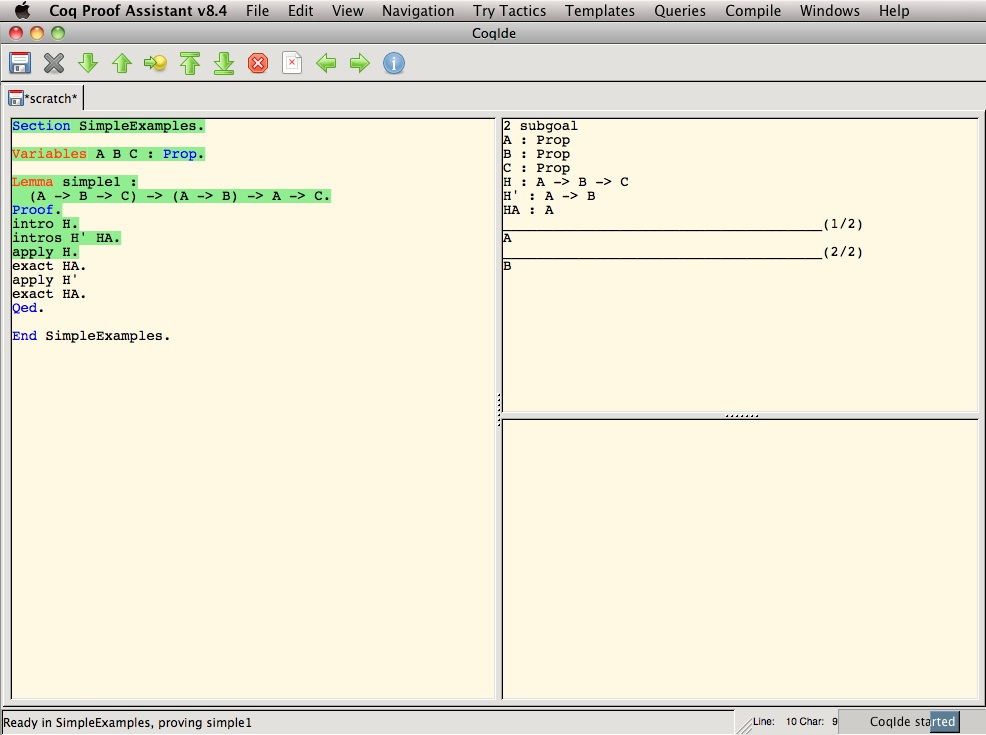
\includegraphics[width=\linewidth]{simple1_1.jpg}
  \caption{CoqIde, displaying the result of entering the tactic ``\texttt{apply H}'' in the top-right panel within the proof of \texttt{(A -> B -> C) -> (A -> B) -> A -> C}.}
  \label{fig:simple1_1}
\end{figure}

\begin{figure}[H]
  \center
  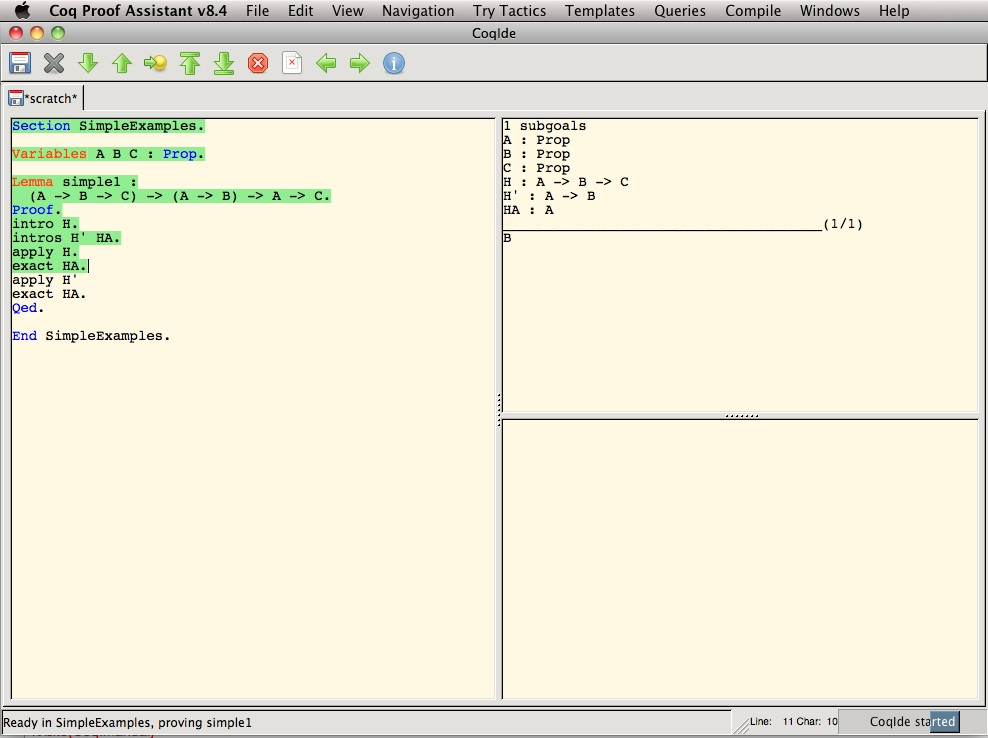
\includegraphics[width=\linewidth]{simple1_2.jpg}
  \caption{CoqIde after moving the end of the evaluated portion of the script forward by one sentence from the state shown in \autoref{fig:simple1_1}.}
  \label{fig:simple1_2}
\end{figure}


Users can extend the highlighted region both forward, to evaluate unhighlighted sentences, and backwards, to undo the effects of evaluation.  Users can instruct the system to extend the highlighting forward by one sentence, to retract it back by one sentence (though in the latest version of Coq, this sometimes will actually move the highlighting back several sentences), to extend or retract it to the cursor, to remove all of it (i.e. retract it to the start of the script), and to extend it to the end of the script.  These instructions can be entered into the system using toolbar buttons, drop-down menu items, or keyboard shortcuts.

\autoref{fig:simple1_1} and \autoref{fig:simple1_2} illustrate some of these points.  In \autoref{fig:simple1_1}, in the top right, we see the the result of evaluating ``\texttt{apply H}''.  In \autoref{fig:simple1_2}, we see the highlighting extended and the result of ``\texttt{exact HA} in the top right, namely the elimination of the first of the two subgoals in \autoref{fig:simple1_1} and the change in focus to the second.

This interface is problematic for novices trying to learn the effects of tactics.  Unfortunately, because the particular example being discussed is so simple, the severity of the problem may not be immediately apparent.  In \autoref{fig:simple1_1}, the two goals resulting from using the tactic ``apply H'' (the statement at the end of the highlighted region) appear to be displayed in the top right panel.  In fact, as mentioned earlier, only the first goal is fully displayed--the context for the second is not.  (In this case, the contexts for both are identical, but this is not always what happens).  To see the context of the second goal, probably the easiest, or at least most natural, thing for the user to do is highlight forward through all the tactics used to prove the first goal (just one tactic here, but potentially many in general).  It is up to the user to determine how far to highlight (or un-highlight, if looking at an earlier sibling goal) by keeping track of the list of goals in the top-right panel.  

In addition to the fact that users must move through the script to fully see siblings, no distinction is made between sibling and non-sibling goals in the list presented.  For instance, instead of using ``\texttt{exact HA}'' to transition to \autoref{fig:simple1_2}, the user could have used a tactic that produced two new goals.  The list of goals would then contain three goals, but only the first two would be siblings.  The user interface leaves it up to the user, however, to determine this by keeping track of the number of goals.\footnote{This sort of debugging gets even harder when one introduces proof automation features that allow combinations of basic tactic use attempts.}

Proof General does introduce a few features not present in CoqIde.  For instance, instead of making the highlighted region un-editable (``locking'' it), typing in the highlighted region retracts the highlighting back to the end of the sentence that is immediately before the cursor.  Unfortunately, these features are not really aimed at showing the effects of tactics.  A third user interface, \textit{Proof Web}\cite{ProofWeb} does make a serious attempt.  ProofWeb, for the most part, is a web-based version of CoqIde.  However, it has a major improvement, shown in the bottom right of \autoref{fig:proofweb}: a visualization of the partially completed proof tree.  

ProofWeb's display of the tree follows the convention where inferences are drawn with a horizontal line separating horizontally listed premises, above, from the conclusion below, and where each horizontal line is labeled with the name of the corresponding inference rule (or, in the case of Coq, by the corresponding tactic name) to the right of the line.  These inferences can be chained together so that the root of the proof tree is drawn at the bottom and the leaves are drawn at the top.  As an example, the portion of the proof tree constructed by ProofWeb that corresponds to ``\texttt{apply H}'' is shown in \autoref{fig:applyH} (the ellipses indicate that the child nodes are still unproved), and \autoref{fig:fulldisplaypartialtree} fully displays the partially completed tree.  The user is able to much more directly see the goal to which \texttt{apply H} is applied and the goals this application produces.

\begin{figure}[H]
  \center
  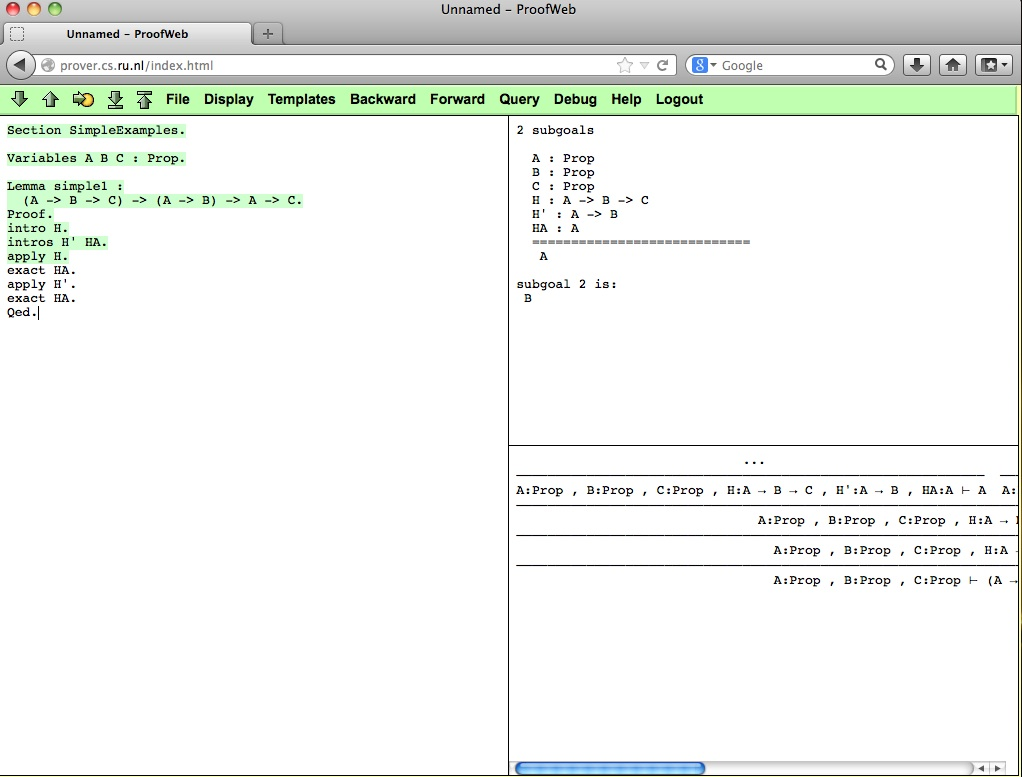
\includegraphics[width=\linewidth]{ProofWeb.jpg}
  \caption{ProofWeb, with a partial proof tree displayed in the bottom right.}
  \label{fig:proofweb}
\end{figure}



Unfortunately, as one can probably already tell, this sort of visualization does not scale particularly well.\footnote{Later in this document I provide what I hope is a clearly better alternative.} Contexts may may have dozens of items, many of which may be much longer than ``\texttt{H : A -> B -> C}'', and the number of nodes in the proof tree may also be very large.  As a result, the user may have to pan around the window to see the effect of a tactic; this is especially likely if one is looking at a tactic used near the root of the tree, since the width of the tree at its leaves forces apart nodes near the root.  Even if the user does not need to pan (ProofWeb has a feature that allows the tree to be displayed in a separate window, which can sometimes make panning unneccessary), the distances at which nodes with sibling and parent-child relationships must sometimes be placed may make it difficult for the user to compare such sequents and to determine if a direct relationship in fact exists (e.g. determine if two sequents that are printed next to one another are siblings or ``cousins'').  The latter task is possibly especially difficult using this visualization since it involves checking for gaps in co-linear line segments and the human brain tends to connect such lines.\footnote{This is the Gestalt law of ``good continuation; see, for instance, \cite{field1993contour}.}  The proof tree visualization, especially if there is a need to pan, is also not particularly helpful in showing the location of the current goal (users may have to search the leaves of the tree to find the leftmost ellipsis).

\begin{figure}[H]
  \center
  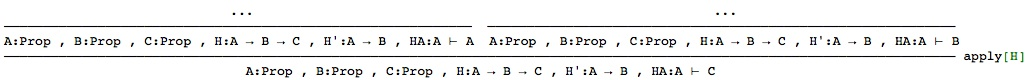
\includegraphics[width=\linewidth]{applyH.jpg}
  \caption{The portion of ProofWeb's tree visualization corresponding to the tactic ``\texttt{apply H}''.}
  \label{fig:applyH}
\end{figure}

\begin{figure}[H]
  \center
  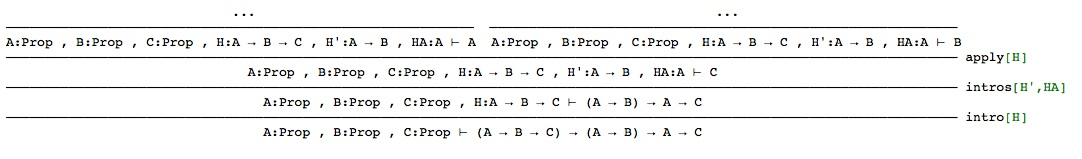
\includegraphics[width=\linewidth]{fullDisplayPartialTree.jpg}
  \caption{The partially completed tree from \autoref{fig:proofweb}, fully displayed.}
  \label{fig:fulldisplaypartialtree}
\end{figure}

The problems with current user interfaces that are discussed above are with respect to the scenario in which a novice user is inspecting an existing proof in order to determine the effects of various tactics under various conditions.  Many other scenarios with overlapping and related challenges also exist.  Such challenges include, but are not limited to,
\begin{itemize}
	\item locating particular items in a context (or in the larger environment)
	\item finding similar nodes in a proof tree
	\item deciding which tactic to apply
	\item keeping track of different proof attempts
	\item optimizing a proof or organizing a set of definitions, theorems and proofs for human understanding
	\item doing all these things efficiently. 
\end{itemize}



%%================================
\section{Coq User Interface Survey}
%%================================
Section \ref{currentUIproblems} described some usability problems that I, as a novice Coq user, noticed.  In this section, I describe an online survey (and its results) that Professor Juan Pablo Hourcade, Professor Aaron Stump, and I, in December 2011, invited subscribers to the Coq-Club mailing list to fill out.  This survey asked Coq users for their opinions and experiences regarding existing Coq user interfaces, and for their ideas regarding new interfaces.  Our motivation was both to validate our own ideas about new Coq user interfaces and to generate new ones.  We received 48 responses, including many detailed responses to the essay questions in the survey.

The survey consisted of 19 questions, of which 13 were multiple choice and the rest short answer or essay. The questions can be divided into three groups:  7 questions asking for background information on the respondent and how the respondent uses Coq, 9 questions asking for various ratings of the interface respondents use, and 3 open-ended questions directly related to the development of new user interfaces.  To these open-ended questions, we received many lengthy and thoughtful responses. \footnote{A more detailed survey report can be found at http://www.cs.uiowa.edu/~baberman/coquisuvey.html.}

The responses to the first group of questions showed a full range of (self-reported) Coq expertise levels, although a majority of responses indicated a high degree of expertise (on a scale going from 1=�novice� to 5=�expert�, 2 respondents rated themselves at level 1, 12 at level 2, 9 at level 3, 17 at level 4, and 8 at level 5).  9 respondents indicated they had been using Coq for less than 1 year, 27 for 1-5 years, 7 for 5-10 years, and 5 for more than 10 years.  Users of Proof General outnumbered users of CoqIDE 31 to 16.  24 respondents indicated using Coq for programming language or program verification research, 10 indicated using Coq for formalization of mathematics, and 8 indicated �teaching.� 

In the second group, to the question ``How satisfied are you with the interface you typically use?'', respondents gave a slightly positive average response (4.6 on a 1 to 7 point scale).  This was somewhat surprising to us at first, but it may have been an artifact of how the the question was asked.  For one thing, we did not present any sort of alternative interface, and current interfaces are, in fact, a significant improvement over the basic command prompt.  A second factor may be that many respondents have become accustomed to their current interface and may have viewed the question as asking how willing they would be to learn to use a new interface.  More than 25\% of respondents, however, did indicate some level of dissatisfaction.  Furthermore, answers to four questions revealed difficult tasks for users.  These questions asked users how difficult it is, using the interface they typically use, to 
\begin{itemize}
\item understand the relationships between subgoals, 
\item switch back and forth between potential proofs of a subgoal, 
\item compare similar subgoals, and 
\item tell what options for proving a subgoal are available. 
\end{itemize}
On a scale where 1=``Very Difficult'' and 7=``Very Easy'', the mean values for the answers to these questions were 2.74, 3.46, 2.35, and 2.57, respectively.   Responses to a fifth question, �How difficult is it for you to (mentally) parse Coq syntax?�, produced a mean value of 5.02 on the same scale, with only 4 responses indicating �Difficult� or �Somewhat difficult�.  Again, this may have been an artifact of the way the question was asked (e.g. to what the task might or might not in comparison be difficult was left unspecified).

In the third group, we received almost 4,500 words (total) in response to the questions  
\begin{itemize}
\item ``What information would you like to have more readily available when working with Coq?'',
\item ``What do you think are the hardest parts of learning interactive theorem proving with Coq?'', and
\item ``What advice/requests/ideas do you have for creating better Coq user interfaces?''
\end{itemize}
Because of this volume, I (very roughly) categorized the responses to each question.

For the first question, the first category was ``library documentation.'' Respondents noted that Coq's ``\texttt{SearchAbout}'' command is a little hard to use, that they would like more simple examples of using Coq commands, that theorem names are not very readable, and that they would like integration of documentation, a la the Eclipse IDE's javadoc support.\footnote{For the reader not familiar with Integrated Development Environments, they are essentially text editors with features specialized to programming in various languages.  Eclipse\cite{Eclipse} is one of the more popular IDEs for Java programming.}  The second category was ``available tactics''/``relevant lemmas, relevant definitions'': respondents wanted the names of previously proved statements they could apply and, additionally, whether a tactic could be used to automatically prove either the the current goal or its negation.  The third category was information on terms, e.g. the type of a term, the value to which it reduces, or other implicit information (such information can already be made available by using commands like ``\texttt{Check}'' and ``\texttt{Print}'').  The fourth category was proof structure, including information on the relationships both between goals within a proof and between theorems and definitions.  Miscellaneous responses included similarities between terms, differences between terms and expected terms, and tactic debugging with custom breakpoints.

For the question ``What do you think are the hardest parts of learning interactive theorem proving with Coq?'', the first category of response was type theory-- that learning the type theory behind Coq is one of the hardest parts.  The second category was with lack of good tutorials.  The third category was that there are numerous poorly documented commands (the need for simple examples was mentioned again).  Finally, the fourth category was proof readability, e.g. lack of support for mathematical notation and proof script organization.

For the question ``What advice/requests/ideas do you have for creating better Coq user interfaces?'', the first category was programming IDE features (e.g. auto-indentation, safe and correct renaming of identifiers, refactoring of tactics and groups of tactics, and background automation).  The second category was proof structure: representing proof structure by, for instance, grouping sibling goals, and allowing more flexibility to the order in which one works on goals.  The third category was syntax, which included having better ways to indicate where one wants to rewrite part of a term or where one wants to unfold a definition and automatic naming of hypotheses.  Some miscellaneous suggestions were to make more use of the mouse, avoid unnecessary re-execution of potentially long-running commands, and to have different editing and presentation tools.   

Even given the responses from self-described novice Coq users, the group of respondents is still heavily biased towards acceptance of arcane, complicated software.  The responses summarized above demonstrate that, even by this group, room for improvement is seen.


%=============================================================================
\chapter{CoqEdit, Proof Previews, and Proof Transitions}
\label{chapter:coqedit}
%=============================================================================

\section{Software Description}

\subsection{Basic CoqEdit}

The basic version of CoqEdit is a jEdit plugin providing a new user interface to Coq that is intended to imitate CoqIDE (see \autoref{fig:simple1_1}), Proof General, and ProofWeb (see \autoref{fig:proofweb}), described in \autoref{currentUIproblems}.  A significant difference between it and these previous user interfaces, however, is the use of two different shades of green, as seen in \autoref{fig:coqedit}:  all sentences highlighted with (some sort of) green are ones that have been successfully evaluated and cached, but the sentence highlighted with dark green has the result of its evaluation displayed in one of the two sub-windows on the right.  The user can move the dark green sentence around in this cached area.   This is in contrast to user interfaces like CoqIDE where there is only one shade of green, the evaluation result displayed on the right is always that of the last green sentence, and there is no caching of output.  Using CoqIDE, to check the result of an sentence evaluated earlier one must actually undo the evaluation of subsequent sentences (Proof General, like CoqEdit, caches evaluated sentence output, but has users hover over the evaluated sentence to see its result).  CoqIDE gets away with this because, frequently, re-evaluating a sentence is instantaneous.  However, this is not always the case, especially when using tactics that automatically search for proofs for goals (in general these are actually semi-decidable).  

\begin{figure}[H]
  \center
  \includegraphics[width=\linewidth]{CoqEdit.jpg}
  \caption{The basic CoqEdit user interface}
  \label{fig:coqedit}
\end{figure}

To move the dark green highlighting forwards or backwards, one can select drop-down menu items (not shown in \autoref{fig:coqedit}, accessible through the ``CoqEdit'' submenu added to jEdit's top-level ``Plugins'' menu.  However, it is expected that generally users will use shortcuts which can be added and customized through the jEdit options menu (e.g. Ctrl-N for ``Forward one sentence'' and Ctrl-P for ``Back one sentence'').  There are 5 other menu items, which I hope are fairly self-explanatory:

\begin{itemize}
\item ``Show CoqEdit Output Panel,''
\item ``Go to cursor,''
\item ``Go to start,''
\item ``Go to end,'' and
\item ``Interrupt evaluation''
\end{itemize}

There are a few details regarding the user interface which may be unclear from the labels.  ``Forward one sentence'' moves the dark green highlighting forward within the light green section \textit{and}, when the dark green sentence is at the end of the green section, extends a purple section forward as seen in \autoref{fig:coqeditpurple}.  This purple section shows the sentence currently being evaluated and the subsequent sentences queued for processing.  

Frequently, evaluation occurs quickly enough that the purple section is invisible, but, as mentioned earlier, long-running and non-terminating commands may be encountered.  For these cases, the ``Interrupt evaluation'' menu item is provided which, in addition to interrupting any current sentence processing, removes all sentences from the queue of sentences to process and removes all purple highlighting.

\begin{figure}[H]
  \center
  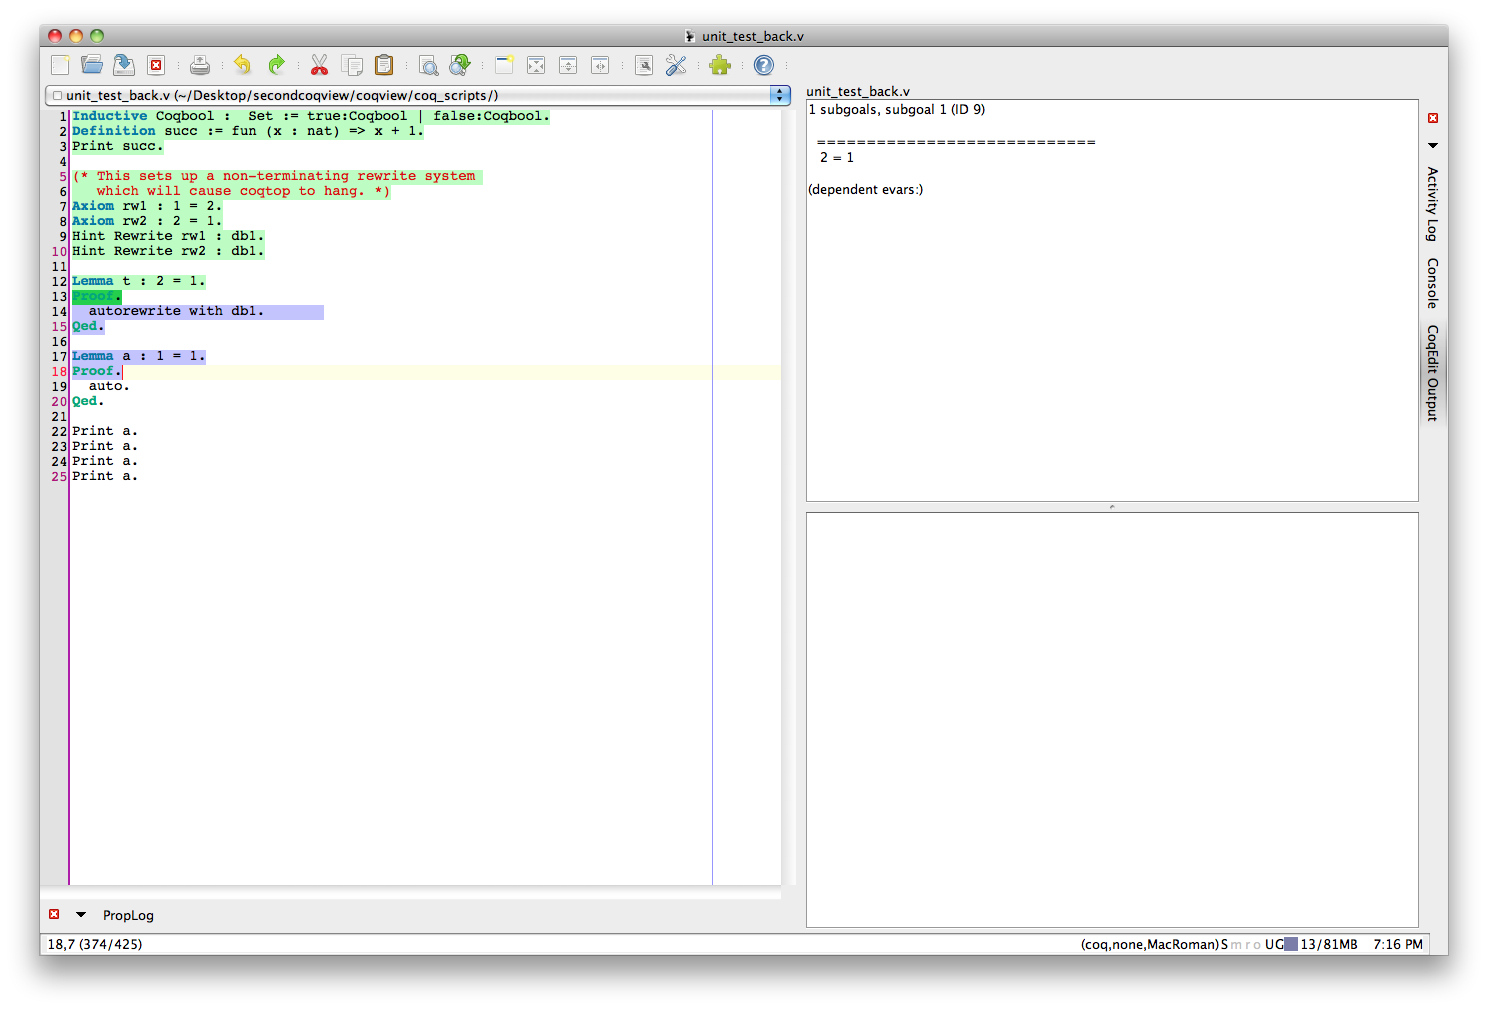
\includegraphics[width=\linewidth]{CoqEditProcessingVisualization.jpg}
  \caption{The basic CoqEdit user interface, when the first sentence highlighted with purple is being evaluated and the subsequent purple-highlighted sentences are queued for processing.  Thanks go to Harley Eades for providing this example of a non-terminating tactic.}
  \label{fig:coqeditpurple}
\end{figure}

The ``Interrupt evaluation'' menu item is not strictly necessary; an equivalent result could be achieved by inserting a character into the first purple sentence (and then deleting that character).  In general, typing into a highlighted region, green, purple, or red (used to indicate errors--see \autoref{fig:coqeditred}), undoes the evaluation/partial processing/queuing of the sentence into (from) which characters were inserted (deleted), and from all subsequent sentences.  To reflect this, the highlighting from these sentences is removed.\footnote{Typing into the sequence of tactics used to prove an earlier theorem or lemma actually causes the highlighting to be moved to just before the start of the lemma; this reflects the behavior of the underlying command line tool.}

\begin{figure}[H]
  \center
  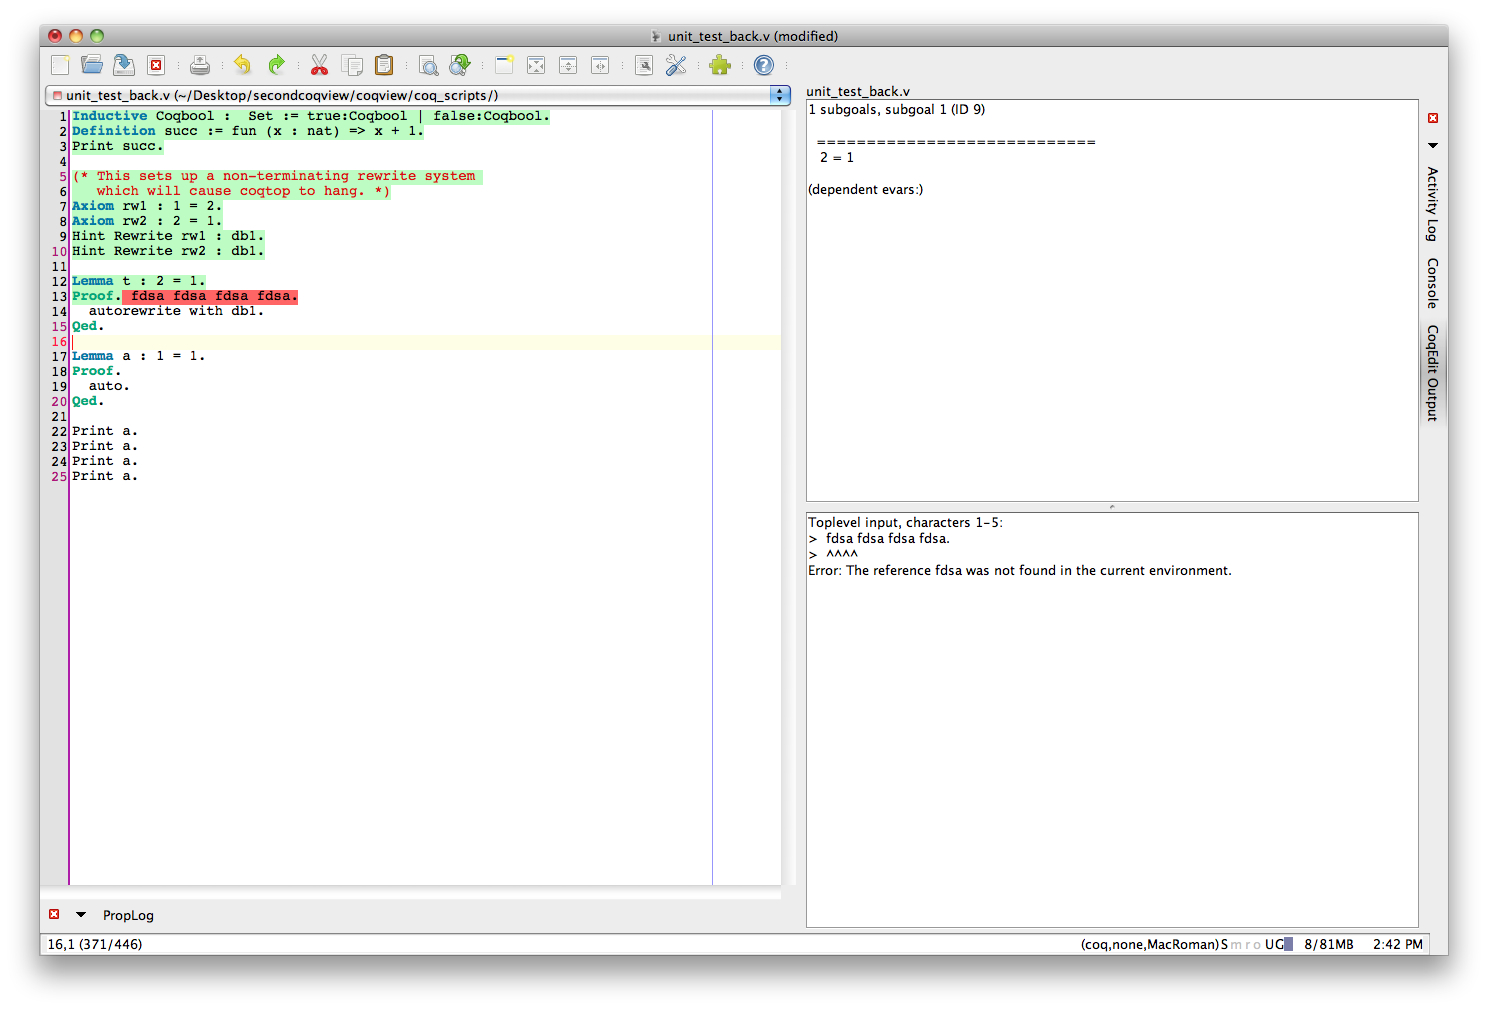
\includegraphics[width=\linewidth]{CoqEditErrorVisualization.jpg}
  \caption{The basic CoqEdit user interface, with an error-producing sentence highlighted in red.}
  \label{fig:coqeditred}
\end{figure}

To try to evaluate all sentences in the buffer, the user can use the ``Go to end'' menu item.  This of course may not always be successful since non-terminating and error sentences may be encountered, as in \autoref{fig:coqeditpurple} and \label{fig:coqeditred}.  Note that when an error is processed, processing stops, the sentences-to-process queue is emptied, and the highlighting is updated to reflect this.  Users are thus informed of incorrect proof attempts.  

``Go to end'' is effectively the same as repeated invoking ``Forward one sentence'' until there are no more sentences that can be queued for evaluation.  Similarly, ``Go to start'' is effectively the same as invoking ``Back one sentence'' repeatedly until the dark green highlighting is at the first sentence of the buffer, and ``Go to cursor'' attempts to move the dark green highlighting forwards or backwards to the sentence containing the cursor by invoking either ``Forward one sentence'' or ``Back one sentence'' repeatedly (when the first purple sentence is evaluated, the dark green highlighting will move to it).  

The navigational commands have the side effect of moving the cursor either to the end of the purple section (if moving forward) or to the end of the dark green sentence.  Moving the cursor in turn has the side effect of automatically scrolling the window so as to keep the cursor (and the most recently changed highlighting) visible.  This turns out to be highly convenient, allowing the user to avoid a large amount of manual scrolling.

As a jEdit plugin, CoqEdit lives in an ecosystem of other plugins which may have specified dependencies on one another.\footnote{If plugin A is specified (in its properties file) as depending on plugin B, then loading plugin A will automatically load plugin B (if it can be found among the downloaded plugins and is not already loaded) and unloading plugin B will (with a warning popup window) unload plugin A.}  One can view jEdit plugins that depend on CoqEdit as plugins to the plugin.  The next subsections describe two ideas for such plugins that were developed, and the next section describes how these ideas were tested with users in an experiment.

\subsection{Proof Transitions}

\subsection{Proof Previews}

\section{Experiment Design, Results, Analysis, and Conclusions}


%=============================================================================
\chapter{Keyboard-Card Menus + Syntax Tree Highlighting, Applied to Fitch-Style Natural Deduction Proofs}
\label{chapter:kcmsth}
%=============================================================================

\section{Keyboard-Card Menus}

  \subsection{Motivation}

  \subsection{Software Description}

  \subsection{Experiment Design, Results, Analysis, and Conclusions}

\section{Syntax Tree Highlighting}

  \subsection{Understanding Syntactic Structure}

  \subsection{Structure Editing}
  
\section{Combined System Description}


%=============================================================================
\chapter{Related Work}
\label{chapter:relatedwork}
%=============================================================================

The need for effective theorem prover user interfaces has been recognized for over 20 years (e.g. \cite{Thery:1992:RTP:142868.143760}) and a series of conferences has even been organized to address this need specifically.\footnote{See http://www.informatik.uni-bremen.de/uitp/ for more information} Many interesting and helpful ideas have been proposed, both for Coq and for related systems.  These ideas vary widely and include integration of Coq, and other theorem provers, with dynamic geometry software \cite{narboux2007graphical,quaresma2007geothms}, easier-to-read declarative languages for proof scripts \cite{corbineau2008declarative}, using wikis for creating proof repositories \cite{corbineau2007cooperative}, and automating the process of using libraries \cite{asperti2010some}.

One approach taken to improve theorem prover user interfaces has been ``Proof by Pointing''\cite{bertot1994proof}, an algorithm to build a proof tree by pointing to portions of a goal.  This was implemented in the \textit{CtCoq} interface \cite{bertot1996ctcoq}, again, later, in the Java-based Pcoq interface \cite{amerkad2001mathematics} and also in the \textit{Jape} system \cite{bornat1999animating}.  Note that some schemes for writing and displaying proofs, notably Fitch style proofs, do not display hypotheses with their conclusion, which may lead to ambiguity when using Proof by Pointing \cite{bornat1997displaying}. 

An example of a recent project is \textit{Panoptes} \cite{farmer2009panoptes}, which allows visualization of proofs produced by the IMPS Interactive Mathematical Proof System.  The system has numerous features allowing users to zoom in on parts of the graph, collapse nodes, rearrange the positions of nodes, label and highlight nodes, and inspect details associated with nodes using pop-up windows.  While these features allow the user to manipulate the presentation of a proof, they do not allow the user to manipulate the proof itself---to change the proof, one must use an Emacs-based environment.

Another significant project is an interactive visualizer for the \textit{ACL2} theorem prover\cite{ACL2}, described in \cite{bajaj2003interactive}.  This tool allows for visualization at three different levels.  It does so first at the level of relationships between theorems and their proofs (the directed acyclic graph describing which lemmas from which libraries are used to prove a given theorem).  Next, it shows a proof tree
%, similar to the visualization given in section \ref{prooftransitions}, 
where a node represents a statement that is being proved using the node's children.  Color coding is used here to indicate the action taken by the prover at a node, and the tree is represented using three-dimensional ``cone trees.''  The contents of the individual nodes, as text, can also be displayed alongside this tree.  At the third level, this text's syntax tree can be visualized (as lines connecting points again, though in a more usual two-dimensional arrangement, and still in contrast with the Syntax Tree Highlighting discussed above).  Selecting text at this level will highlight the corresponding portion of the tree visualization.  The system also supports textual pattern matching, where the degree of matching is indicated by the color of the text and the tree visualization.  Both at this level and at the proof structure level (i.e. the second level) the system is capable of zooming and panning, and, at the proof structure level, rotating is also possible.

A few other significant projects aiming to improve the presentation of machine-checked proofs include \textit{Proviola}, which allows users to move through a proof script displayed on a web page and view the results that Coq would produce \cite{tankink2012narrating}; an ``Interactive Derivation Viewer'' for visualizing derivations written in the TPTP language \cite{trac2007interactive}; the LOUI interface for the OMEGA proof assistant, featuring graphical visualization, term browsing, and natural language proof presentation \cite{siekmann1999loui}; and the Tecton system, featuring tree visualization combined with hypertext navigation of nodes \cite{kapur1994overview}.  Theoretical and methodological work has also been done and can be seen in \cite{eastaughffe1998support,bertot1998generic,luth1999functional,volker2004thoughts,geuvers2009proof}, and \cite{luth2009user}.  Work aimed at making ITPs more suitable for novices and educational settings includes \cite{tsovaltzi2003approach,meier2004adaptable,narboux2007graphical,billingsley2007student,dillinger2007acl2s,hendriks2010teaching,schreiner2009risc} and \cite{pierce2010proofassist}.

In addition to previous work specifically on theorem prover user interfaces, it is important to consider more general human-computer interaction research and research on software development tools.  Starting with the latter, one can consider the data of \cite{murphy2006java} showing that the Eclipse IDE's ``rename,'' ``move,'' ``extract'', and ``inline'' refactoring commands are in fact used by many programmers and are frequently invoked via key bindings.  The data also shows that a large percentage of \textit{all} commands executed by developers using the IDE extensively were invoked via key bindings, and one of the top commands was ``content assist'', which suggests possible text to insert (similar to Proof Previews, though it does not show the effects of evaluating this text).  One may also note, here, the existence of various lines of work, e.g. the \textit{Frama-C} \cite{FramaC} project, aimed at integrating theorem proving and programming within IDEs.

In addition to IDEs, we may consider software visualization tools:  \cite{bassil2001software} reports on a survey of users of software visualization tools such as \textit{daVinci} (now called \textit{uDraw(Graph)}), \textit{GraphViz}, \textit{Grasp} (now \textit{jGrasp}), and \textit{Tom Sawyer Software}--more than 40 different tools altogether.  Some of the ``functional aspects'' of the software visualization tools that were considered most useful, and that might also have useful analogs in theorem prover user interfaces, were ``search tools for graphical and/or textual elements'', ``hierarchical representations'' and ``navigation across hierarchies'', ``use of colors'', and ``easy access, from the symbol list, to the corresponding source code.''  Among functional aspects considered least useful were ``3D representations and layouts, and virtual reality techniques'' and ``animation effects'', though the later was considered ``quite useful'' when the software was implemented in a declarative language.  Software visualization tools were considered beneficial in increasing productivity and managing complexity, and were considered particularly important in the ``software comprehension process.''

A survey and taxonomy of software visualization is presented in \cite{caserta2011visualization}.  Similar to \cite{bajaj2003interactive}, it divides tools into three groups according to their use at three different levels of abstraction: line, class, and architecture.  They also differentiate between tools used for visualizing code at a particular time and those that allow for visualization of the evolution of software.  Many of the techniques used by these tools could be applied to visualization for interactive theorem provers.  \textit{Seesoft} \cite{eick1992seesoft}, for instance, miniaturizes lines of code with lines of color-coded pixels, and \textit{sv3D} \cite{marcus20033d} extends this idea using three-dimensional arrays of blocks where information about lines of code is encoded in the height and color of the blocks.  Other techniques potentially useful for interactive theorem prover user interfaces include using animation and color gradients to show the direction of relationships between software components \cite{alam2007evospaces,holten2006hierarchical} and using texture and 3D object primitives called ``geons'' to encode additional information \cite{holten2005visual,irani2001using}.

The more general human-computer interaction literature on tree visualization is quite extensive--many techniques have been developed.  Four different ``common layouts'' are listed in \cite{holten2006hierarchical}: rooted tree
%(the node layout presented, for instance, in \autoref{fig:similarnodes}, with 
(child nodes arranged on a horizontal line above or below their parents), radial trees (nodes of each level of the tree are arranged in concentric circles, with the root node at the center, its children at the first circle out, their children at the next circle out, etc.), balloon trees (each parent's child nodes are arranged radially around the parent), and treemaps (which divide a rectangle into smaller and smaller rectangles with the largest rectangle representing the root of the tree and the smallest representing the leaves, and where division of the rectangles switches between using horizontal and vertical lines when going between tree levels; these were developed in \cite{shneiderman1992tree}).  These common layouts have been extended in various ways.  For instance, \cite{nguyen2002space} describes a space-optimized version of balloon trees and \cite{van1999cushion} describes the the addition of gradients to the rectangles in treemap visualizations, making the structure of the tree easier to see.

\cite{katifori2007ontology} presents an extensive review of tree visualization techniques.  Along with classifying visualizations as 2D or 3D (or 2.5D when no movement in or manipulation of a 3D visualization is allowed), it divides the visualizations into six overlapping categories: indented list, node-link and tree, zoomable, space-filling, focus+context or distortion, and three-dimensional information landscapes.  Indented lists can be seen in file system browsers, e.g. \textit{Microsoft Windows}' \textit{Explorer}, the rooted and radial trees mentioned in \cite{holten2006hierarchical} as common layouts are ``node-line and tree'' type, and treemaps are an example of the space-filling type.  An example of a zoomable visualization is \textit{Grokker} \cite{rivadeneira2003study} which allows users to click and expand nested circles.  An example of the focus+context or distortion category is the \textit{Hyperbolic Browser} \cite{lamping1996hyperbolic} which magnifies and centers on the area around a selected node in a radial layout.  An example of a three-dimensional information landscape is the \textit{Harmony Information Landscape} \cite{eyl1995harmony}.


%=============================================================================
\chapter{Summary and Conclusions}
%=============================================================================

%=============================================================================
% \appendix
% %=============================================================================
% 
% %=============================================================================
% \chapter{Sample Appendix}
% 
% \section{Appendix One}
% \blindtext
% 
% \section{Appendix Two}
% \blindtext
% 
% %=============================================================================
% \chapter{Another Appendix}
% 
% \section{Appendix Three}
% \blindtext
% 

%=============================================================================
% bibliography
%=============================================================================
\interlinepenalty=10000	% prevents bib items from splitting across pages
\bibliographystyle{uithesis}
\bibliography{thesis}

\end{document}
